\section{Einf"uhrung}
Programmgesteuerte Datenverarbeitungsanlagen werden allgemein als Rechner oder Computer bezeichnet. Im folgenden Bild ist die Grundstruktur einer programmgesteuerten Datenverarbeitungsanlage zu sehen.

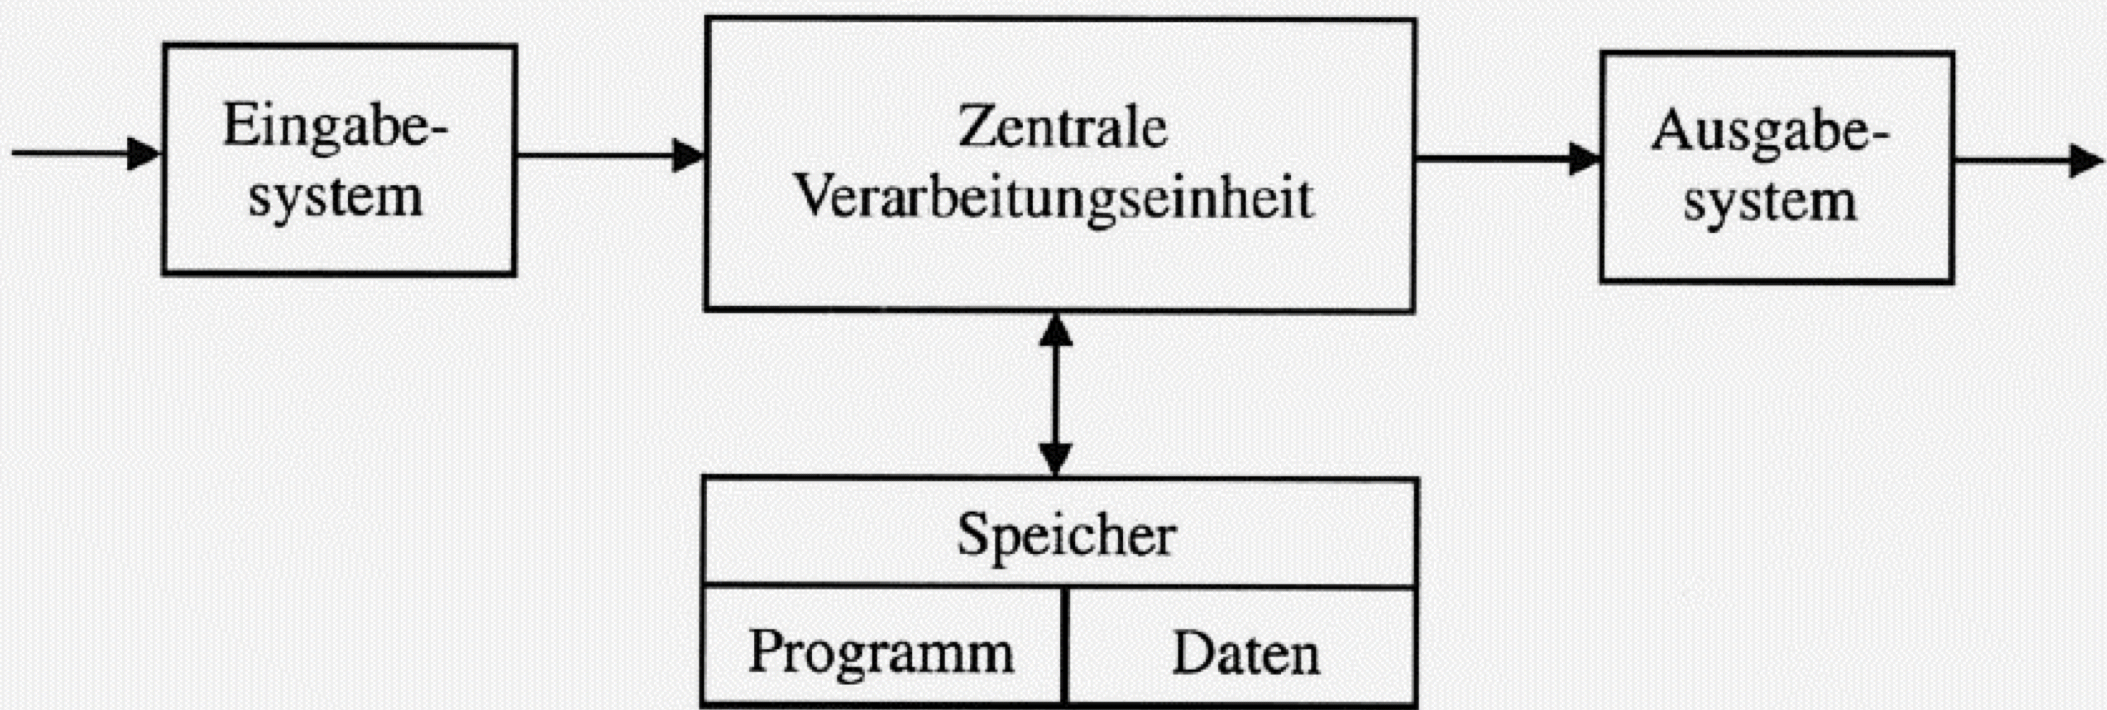
\includegraphics[width = 7cm]{pics/Datenverarbeitungsanlage}

\subsection{Moore's Law}
Moore's Law sagt aus, dass sich die Komplexit"at integrierter Schaltkreise regelm"assig verdoppelt, je nach Quelle werden 12 bis 24 Monate als Zeitraum genannt.

\subsection{Eingebettete Systeme}
\vspace{-4ex}
\begin{minipage}[c]{10cm}
\vspace{-2ex}
Heute sind weit "uber 90\% aller Computer als eingebettete Systeme realisiert, das heisst sie sind in Produkten wie zum Beispiel Haushaltsger"aten, Autos oder Fertigungszellen integriert.

Eingebettet Systeme (Embedded Systems) stellen stets ein Kombination aus Hard- und Softwarekomponenten dar, die in einem technischen Kontext (Prozess, Anlage) eingebunden sind.
\end{minipage}
%
\begin{minipage}{0.5cm}
	\ \
\end{minipage}
\begin{minipage}[c]{6cm}
	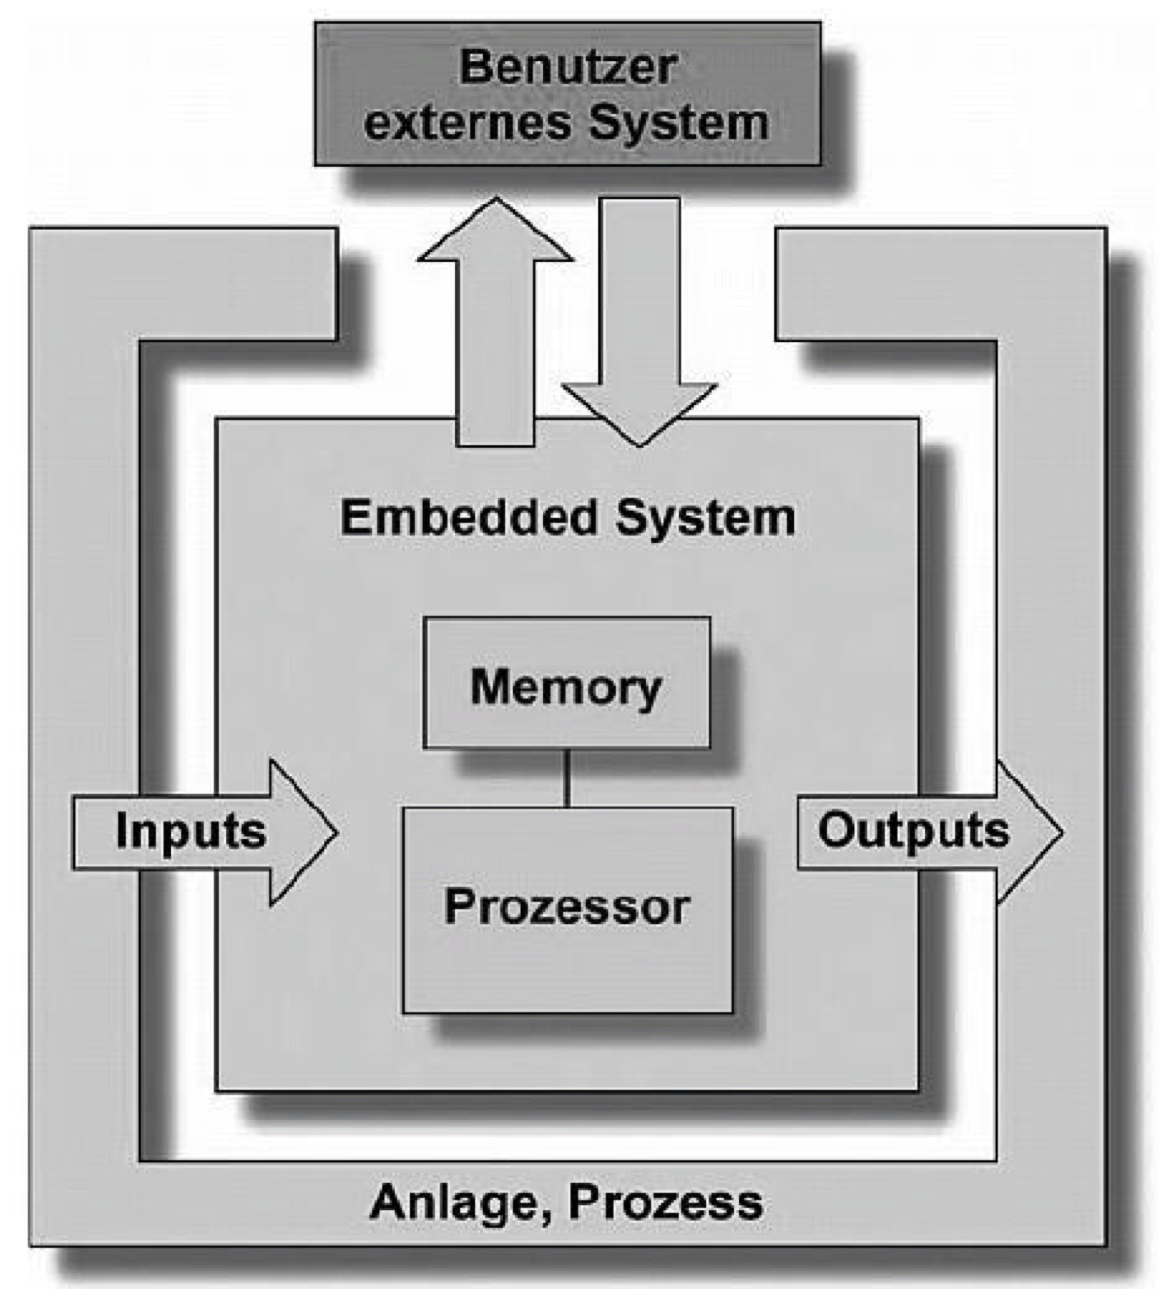
\includegraphics[width=3.5cm]{pics/Embedded-System}
\end{minipage}

\subsection{Bestandteile eine Mikrocomputers}
Ein Mikrocomputer besteht aus einer Zentraleinheit, aus Speicherelementen und aus Eingabe- und Ausgabe-Einheiten sowie aus einem Verbindungssystem.

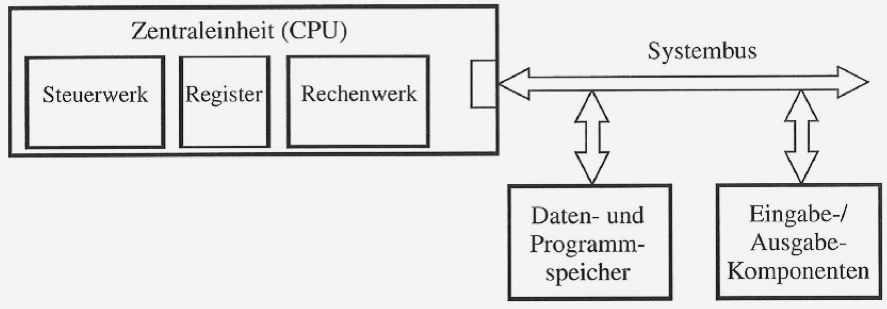
\includegraphics[width = 8cm]{pics/Mikrocomputer}

\begin{minipage}[t]{8.5cm}
	\subsubsection{CPU (Central Processing Unit)}
	Die CPU "ubernimmt als zentrale Berarbeitungseinheit die Datenverarbeitung als auch die Koordination aller computerinternen Aktivit"aten\\
	
	\subsubsection{Eingabe-/ Ausgabe-Einheiten}
	Sie dienen als Schnittstelle zur Aussenwelt. Die Anzahl und konkrete Konfiguration h"angt direkt vom Einsatz und Zweck ab.\\
	
	\subsubsection{Master-Slave-Prinzip}
	Die CPU steuert als Master aktiv alle Abl"aufe und Datentransporte. Speicher und periphere Komponenten arbeiten als Slave und werden normalerweise nur auf Aufforderung durch die CPU aktiv.
\end{minipage}
%
\begin{minipage}{1cm}
	\ \
\end{minipage}
%
\begin{minipage}[t]{8.5cm}
	\subsubsection{Speicher (Memory)}
	Der Speicher nimmt die zu verarbeitenden Daten, das Programm und weitere Informationen w"ahrend des gesamten Programmablaufs auf und stellt diese auf Anforderungen nach Bedarf zur Verf"ugung.\\
	
	\subsubsection{Systembus}
	Der Systembus dient als Verbindungszweig zwischen den Komponenten des Mikrocomputers. Prinzipiell funktioniert die Ablaufsteuerung auf dem Systembus nach einem Matser-Slave-Prinzip.\\
	
	\subsubsection{Interrupt-Konzept}
	Ist eine Erweiterung des Master-Slave-Prinzip, bei der periphere Slave-Einheiten eine Bedienungsanforderung (Interrupt-Request) bei der CPU anmelden k"onnen. Die CPU entscheidet "uber die Ber"ucksichtigung dieser Anforderung und den Zeitpunkt der Bearbeitung.
\end{minipage}

\subsection{Rechnerarchitekturen}
Die Art der Topologie (Zusammenschaltung) der verschiedenen Komponenten in einem Mikroprozessorsystem wird als Rechnerarchitektur bezeichnet.

\begin{minipage}{9cm}
	\subsubsection{Von-Neumann-Architektur}
Ein gemeinsamer Speicher f"ur Programme und Daten ist an einem Systembus angeschlossen. Damit steht nur ein Datenpfad f"ur Programm- und Dateninformationen zur Verf"ugung.

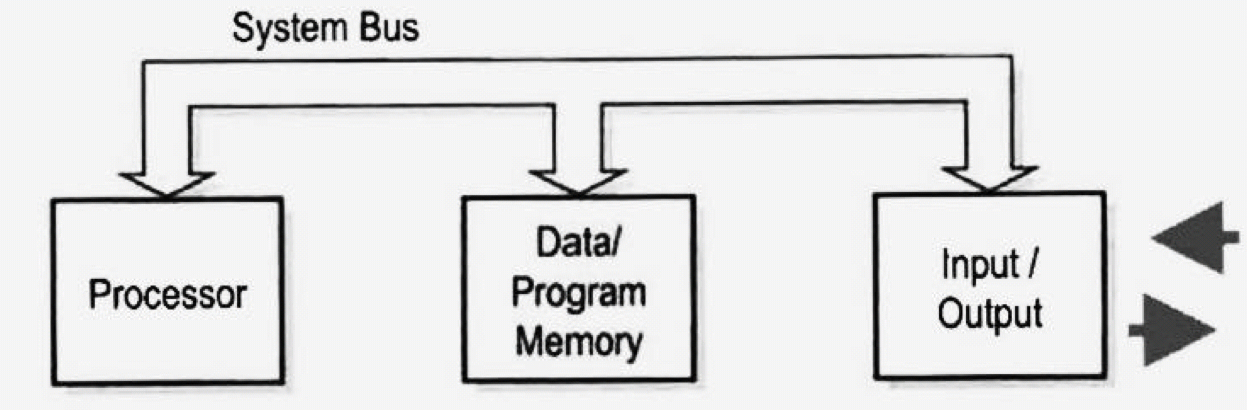
\includegraphics[width = 7cm]{pics/Von-Neumann-Architektur}
\end{minipage}
%
\begin{minipage}{0.5cm}
	\ \
\end{minipage}
%
\begin{minipage}{9cm}
	\subsubsection{Harvard-Architektur}
	Daten- und Programmspeicher sind getrennt ausgef"uhrt und "uber separate Busse an die CPU gekoppelt $\Rightarrow$ zeitgleiche "Ubertragung von Programm- und Dateninformationen.
	
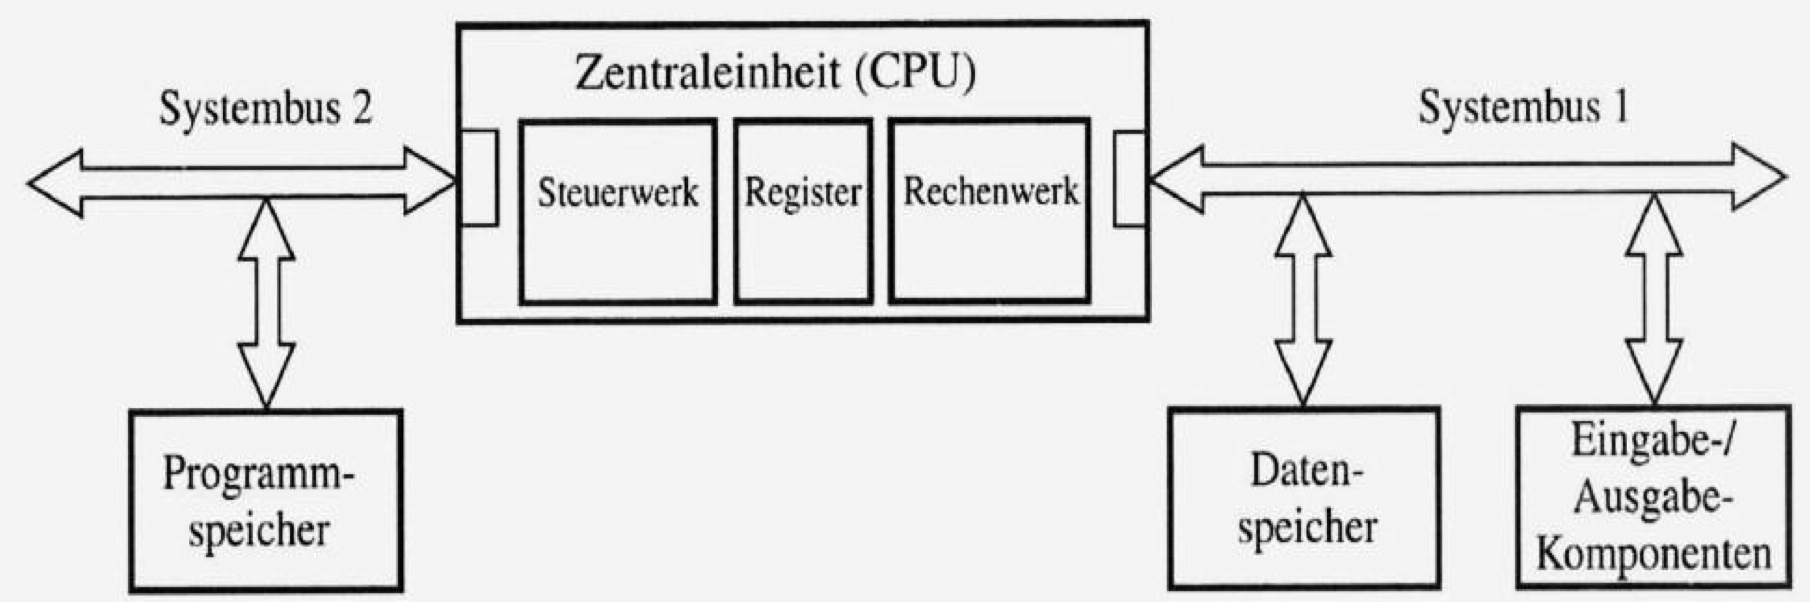
\includegraphics[width = 8cm]{pics/Harvard-Architektur}
\end{minipage}

\subsection{Mikroprozesssortechnik}
\begin{minipage}{11cm}
	Die \textbf{Mikroprozessortechnik} befasst sich mit der Architektur, der Entwicklung, der Implementierung, dem Bau, der Programmierung und dem Einsatz von Mikroprozessoren.

Ein \textbf{Mikroprozessor} ($\mu$P) ist die auf einem Chip realisierte CPU eines Computersystems.

Eine \textbf{Mikroarchitektur} bezeichnet die Implementierung einer Prozessorarchitektur ein einer speziellen Verk"orperung der Architektur - also in einem Mikroprozessor.
\end{minipage}
%
\begin{minipage}{0.5cm}
	\ \
\end{minipage}
%
\begin{minipage}{7cm}
	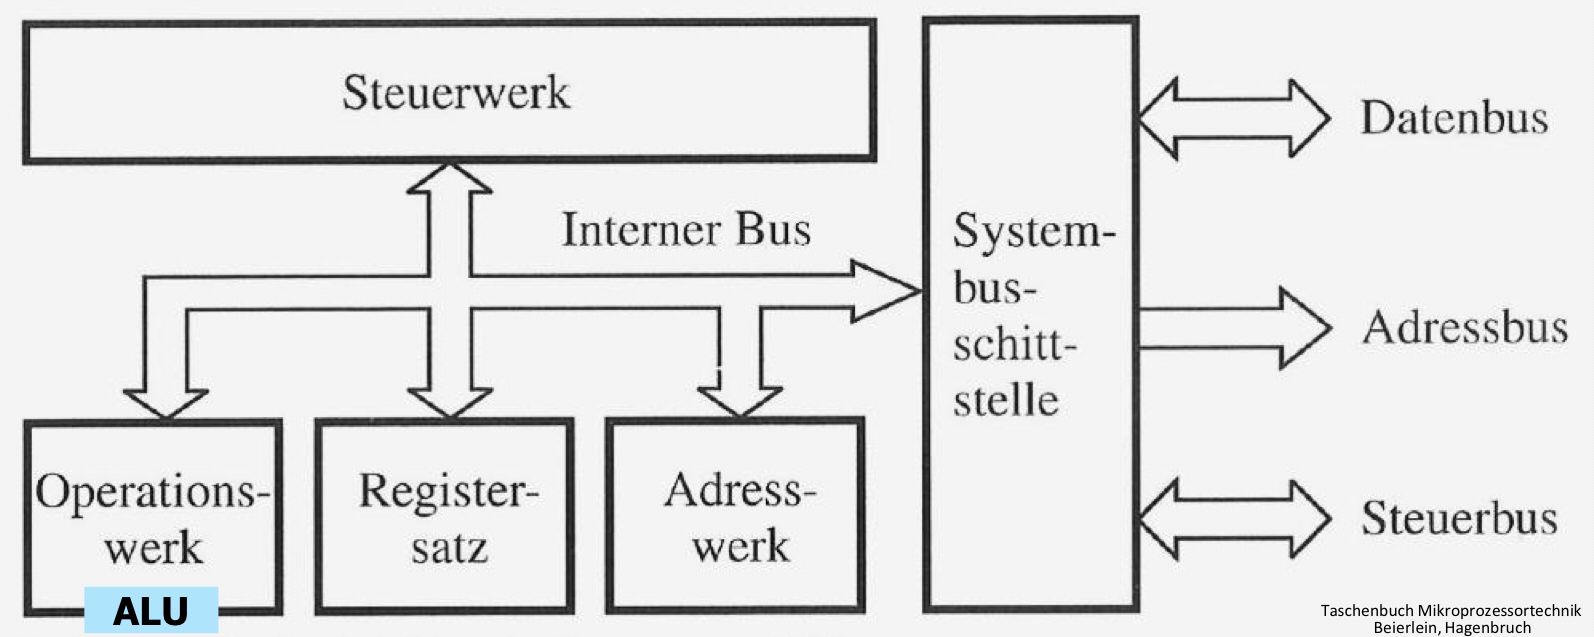
\includegraphics[width=7cm]{pics/CPU}
\end{minipage}

\subsection{Differenzierung von Mikroprozessoren}
Mikroprozessoren unterscheiden sich durch zahlreiche Parameter und Architekturmerkmale. Es gibt f"unf Hauptgruppen.
\textbf{Standard-Mikroprozessoren} sind f"ur den allgemeinen Einsatz z.B. f"ur Drucker, Workstations usw.

\textbf{Hochleistungs-Mikroprozessoren} f"ur Computer mit sehr hoher Verarbeitungsleistung (z.B. f"ur Grossrechner, Netzwerkkomponenten)

\begin{minipage}{9cm}
\subsubsection{Mikrocontroller ($\mu$C)}
	Mikrokontroller sind vollst"andige Mikrorechnersysteme auf einem Chip. Sie beinhalten Speicher Peripherien, CPU und Speicher.
	Sie werden f"ur Automatisierungen, f"ur die Medizintechnik und f"ur viele weitere Sachen verwendet.\\
	\end{minipage}
%
\begin{minipage}{0.5cm}
	\ \
\end{minipage}
%
\begin{minipage}{9cm}
	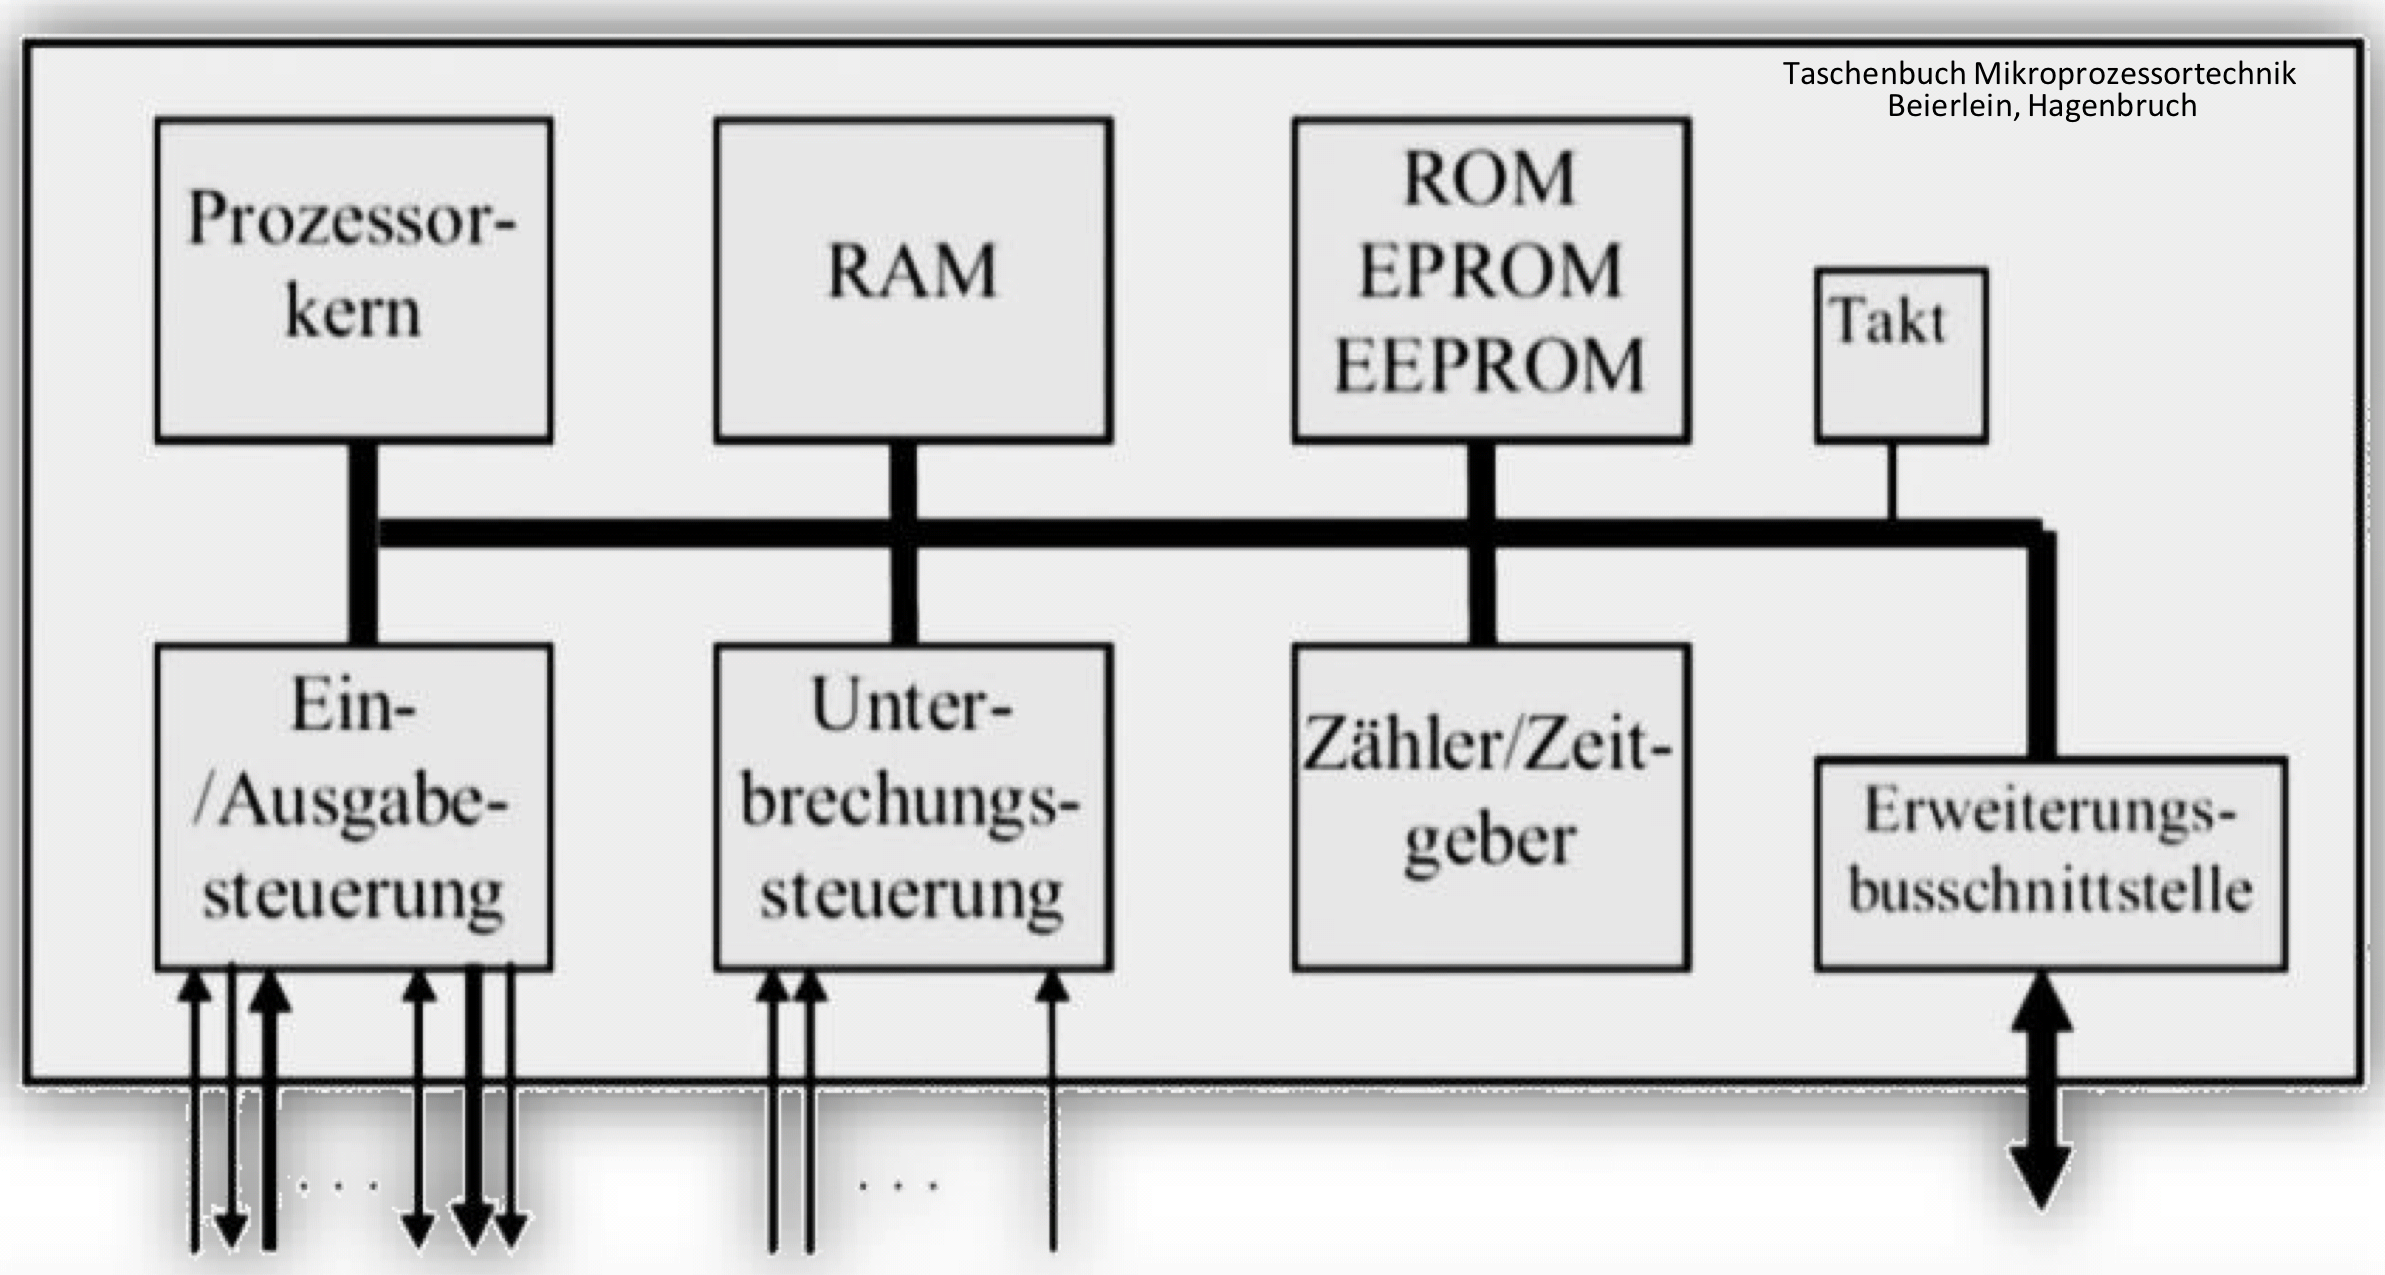
\includegraphics[width=5cm]{pics/Mikrokontroller}
\end{minipage}

\begin{minipage}{9cm}
	\subsubsection{Digitale Signalprozessoren (DSP)}
	Digitale Signalprozessoren sind Mikroprozessoren welche f"ur die schnelle Verarbeitung von mathematischen Befehle und f"ur die Bearbeitung komplexer Algorithmen von digitalisierten Analogsignalen optimiert sind.
\end{minipage}
%
\begin{minipage}{0.5cm}
	\ \
\end{minipage}
%
\begin{minipage}{9cm}
	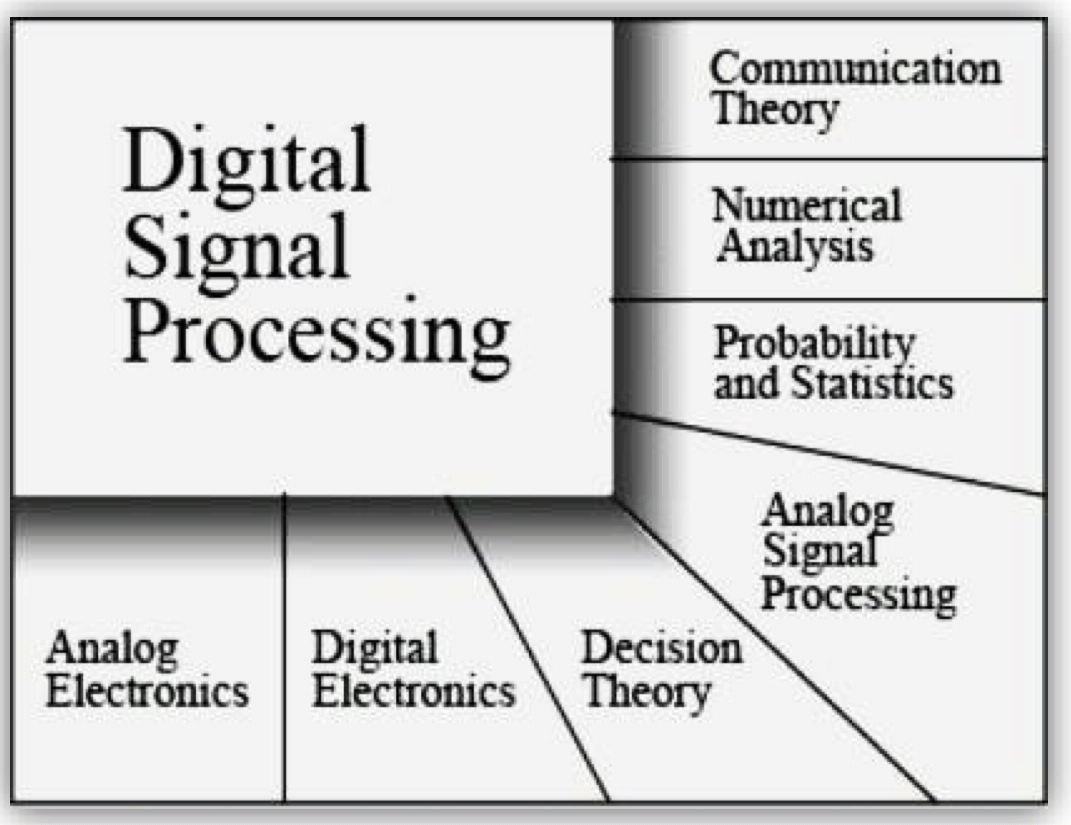
\includegraphics[width=3cm]{pics/Digitale-Signalprozessoren}
\end{minipage}

\subsubsection{Software-Prozessorkern}
	F"ur \textbf{ASIC} (Application-Specific Integrated Circuit) und \textbf{FPGA} (Field Programmable Gate Array) stehen zahlreiche CPU-Designs in Form von Software-Bibliotheken zur Verf"ugung. Solche Software-Prozessorkerne (Soft-Core) erm"oglichen die Realisierung kompletter Systeme auf einem Chip.

\textbf{Systems on Chip} (SoC) sind komplexe Systeme, die eine oder mehrere Verarbeitungseinheiten (CPUs), Programm- und Datenspeicher sowie vielf"altige analoge und digitale Funktionseinheiten auf einem Chip enthalten.

Als \textbf{SoPC} (System-on-Programmable-Chip) bezeichnet die Technologie, ein SoC nicht auf einem ASIC sondern mittels eines programmierbaren Hardware-Bausteins (z.B. FPGA) zu realisieren.

\subsection{Ausgew"ahlte Architekturmerkmale}
\begin{minipage}{14.5cm}
	Das \textbf{Programmiermodell} fasst wichtige Teile der Mikroprozessorarchitektur zusammen und spiegelt die Struktur des Prozessors wieder.

	Bei der Speicheradressierung gibt es das \textbf{Big-Endian- /Little-Endian-Format}, wobei bei der Little-Endian-Formatierung das LSB die Startadresse festlegt und bei der Big-Endian-Formatierung legt das MSB die Startadresse fest.

	Zudem gibt es noch weitere Architekturmerkmale wie Programmierbarkeit des Systemtaktes, ausf"uhrung der Recheneinheit, Taktfrequenz, Cache-Speicher On-CHip, Konfigurierbarkeit von Komponenten des Mikroprozessors usw.
\end{minipage}
%
\begin{minipage}{0.5cm}
	\ \
\end{minipage}
%
\begin{minipage}{4cm}
	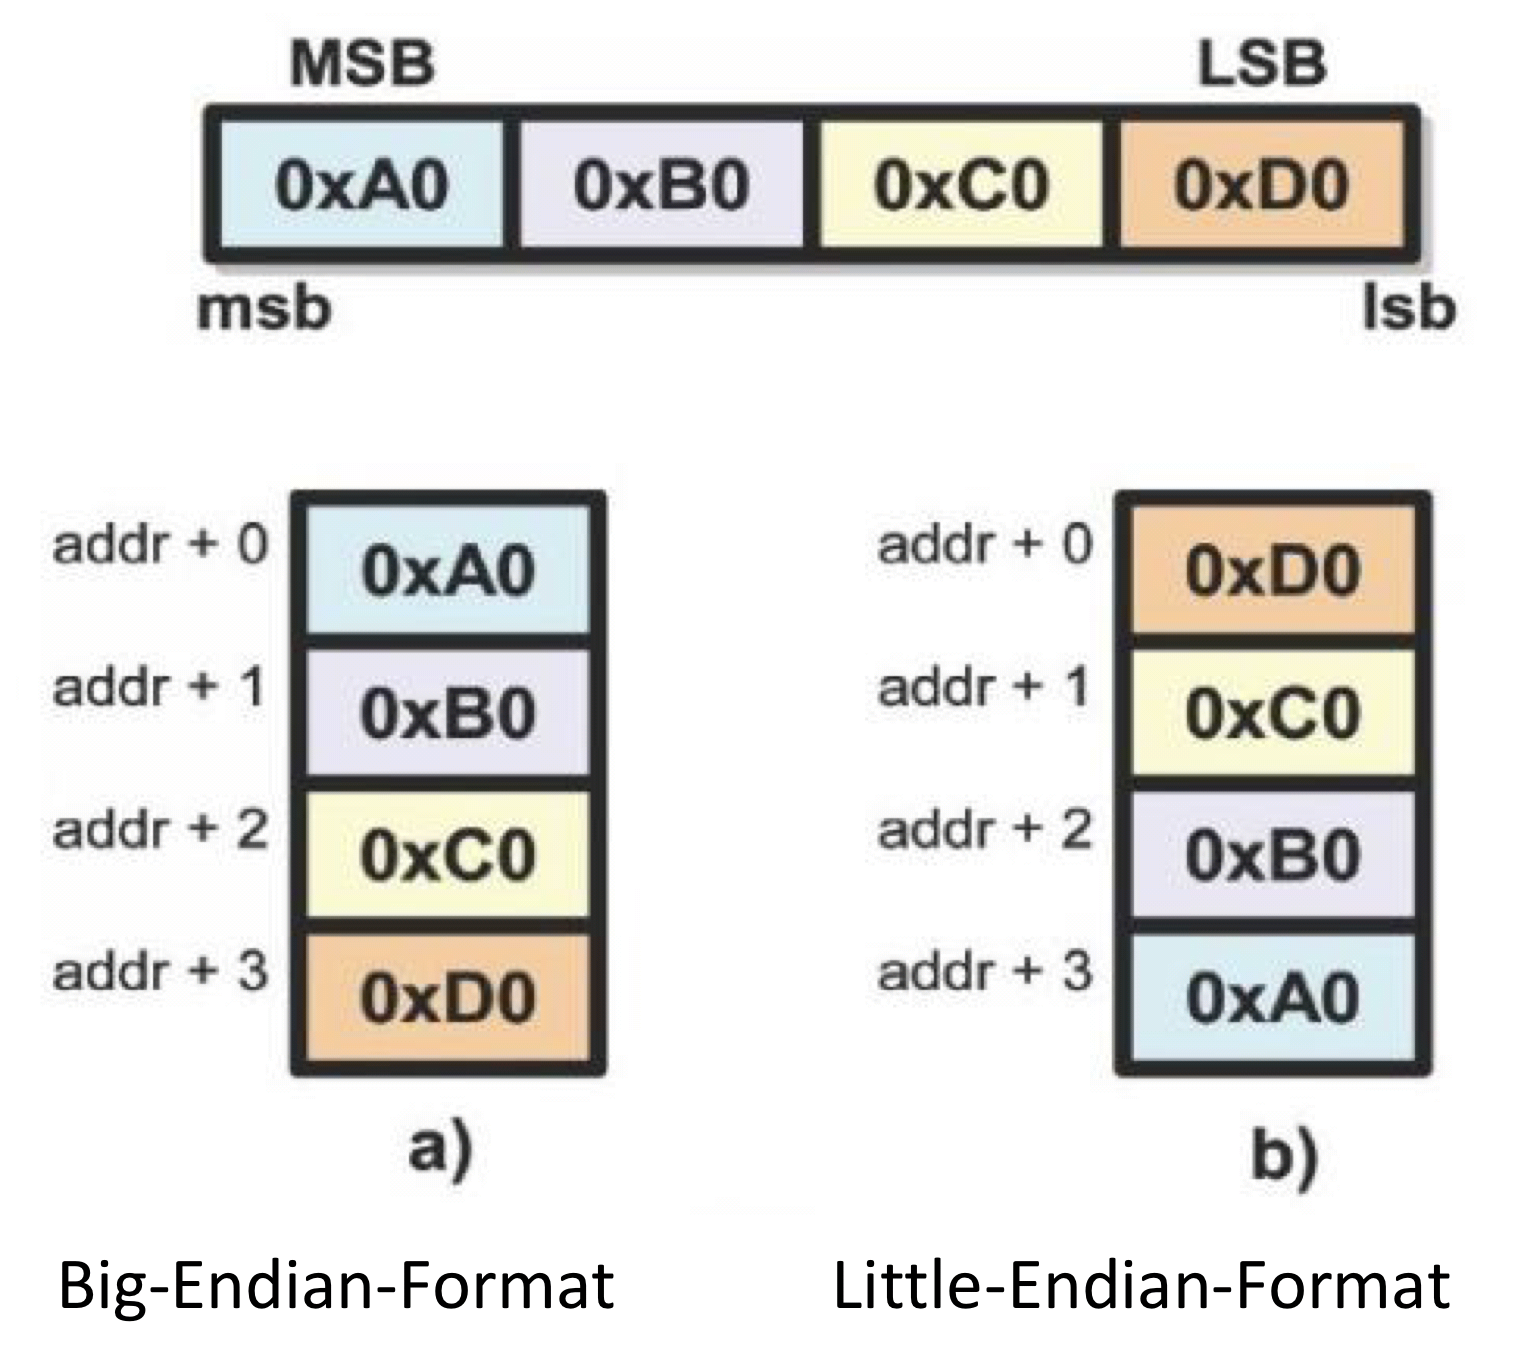
\includegraphics[width=4cm]{pics/Big-Endian_Little-Endian}
\end{minipage}

